\documentclass[12pt,a4paper]{article}
\usepackage[utf8]{inputenc}
\usepackage[french]{babel}
\usepackage[colorlinks=true,linkcolor=black,linktoc=all]{hyperref}
\usepackage[linesnumbered, ruled, french,onelanguage]{algorithm2e}
\usepackage{graphicx}
\usepackage[left=2cm,right=2cm,top=2cm,bottom=2cm]{geometry}
\usepackage{colortbl}
\usepackage[nottoc]{tocbibind}
\usepackage{textcomp}
\newcommand\tab[1][0.65cm]{\hspace*{#1}}

\begin{document}
\begin{titlepage}
	\begin{figure}
	\centering
	\begin{minipage}{.5\textwidth}
  	
\includegraphics[width=.5\linewidth]{ISIR.png}
	\end{minipage}%
	\begin{minipage}{.5\textwidth}
  	\centering
  	
\includegraphics[width=.8\linewidth]{SU.jpg}
	\end{minipage}
	\end{figure}
	\centering
	\par
	{\scshape\large \  \par}
	\vspace{2.5cm}
	{\huge\bfseries Rapport de stage :\\
		Design, Réalisation, et Évaluation des techniques d'interaction\par}
	\vspace{2cm}
	{\Large\ B. Thanh Luong \par}
	\vspace{0.5cm}
	{$1^{\texttt{\footnotesize ère}}$ année Spécialité ANDROIDE\\}
	{Année universitaire 2017 - 2018}
	\vfill
	\begin{minipage}{.5\textwidth}
	\centering
  	Responsables pédagogiques :\par
	Pierre Fouilhoux : \href{mailto:pierre.fouilhoux@lip6.fr}{pierre.fouilhoux@lip6.fr}\par
	Viet Hung Nguyen : \href{mailto:hung.nguyen@lip6.fr}{hung.nguyen@lip6.fr}\par
	\end{minipage}%
	\begin{minipage}{.5\textwidth}
  	\centering
  	Tuteurs :\par
	Gilles Bailly : \href{mailto:gilles.bailly@upmc.fr}{gilles.bailly@upmc.fr}\par
	Sylvain Malacria : \href{mailto:sylvain.malacria@inria.fr}{sylvain.malacria@inria.fr}
	\end{minipage}
	\vfill

% Bottom of the page
	{\large août 2018\par}
\end{titlepage}
{\huge \textbf{Remerciements}}\\
\vspace{0.5cm}

Je tiens à remercier tout le personnel de l'ISIR pour son accueil
chaleureux ainsi que toutes les personnes qui ont contribué au succès de tout au long de mon stage et les diverses connaissances qu'elles ont partagé avec moi durant toute cette période.
\vspace{0.5cm}

Tout d'abord, j'adresse mes remerciements à tous les membres du groupe HCI de l'équipe Interaction, à savoir mes tuteurs M. Gilles Bailly et M. Sylvain Malacria de l'équipe Loki du centre Inria Lille pour leur disponibilité et leurs conseils.
\vspace{0.5cm}

Je tiens ensuite à remercier M. Cédric Honnet et M. Marc Teyssier qui ont également été très disponible pour les matériels informatiques.
\vspace{0.5cm}

Enfin, je tiens à remercier les responsables du Master ANDROÏDE qui m'ont permis d'effectuer ce stage afin de compléter ma formation d'ingénieur avec leurs cours. Ces connaissances complémentaires m'ont permis d'être encore plus performant lors de mon stage en entreprise et de trouver des
solutions auxquelles je n'aurais peut être pas pensé auparavant.
\newpage
{\huge \textbf{Résumé}}\\
\vspace{0.5cm}

Dans ce rapport de stage sont présentées les différentes étapes de développement des techniques d'interaction et de leur évaluation via une application d'édition de texte. Cette application a pour but de
permettre aux chercheur du domaine interaction d'étudier des comportements d'utilisateurs sur les techniques différentes. L'application fournit 4 techniques d'utilisation des raccourcis dont une est déjà implémentée. Les techniques d'interaction permettent aux utilisateurs d'avoir une nouvelle perception du lien entre les commandes et leurs raccourcis. Le but est d'avoir une vue d'ensemble sur ces techniques et de déduire la meilleure parmi celles proposées. Parmi les 4 techniques, deux techniques sont visuelles et deux sont physiques.

Ce stage se déroule du 6 juin au 31 juillet 2018 à l'ISIR qui est un laboratoire de recherche commune à Sorbonne Université et au Centre National de la Recherche Scientifique (CNRS).
\newpage
\tableofcontents
\newpage
\section{Introduction}
Dans le cadre de ma première année de Master Informatique spécialité ANDROÏDE à Sorbonne Université, je souhaite effectuer un stage d'été d'une durée de 2 mois. Il me permet d'être formé au sein d'un laboratoire dans le but d'acquérir des connaissances sur un secteur d'activité, tout en me permettant de mettre en pratique les connaissances théoriques que j'ai acquises lors de mon cursus.

Dans ce rapport, je présente mon environnement de travail ainsi que la mission principale que j'ai réalisée au sein du laboratoire ISIR, à savoir le développement des techniques d'interaction et leur évaluation.
\section{Environnement}
\subsection{Le laboratoire}
\begin{center}
	
\includegraphics[width=.3\linewidth]{ISIR.png}
\end{center}

L'Institut des Systèmes Intelligents et de Robotique (ISIR), qui a été créé au $1^{\texttt{\footnotesize er}}$ janvier 2007, est un laboratoire de recherche pluridisciplinaire qui rassemble des chercheurs et enseignants-chercheurs relevant de différentes disciplines des Sciences de l’Ingénieur et de l’Information ainsi que des Sciences du Vivant.

L’ISIR est une Unité Mixte de Recherche (UMR7222) commune à Sorbonne Université et au Centre National de la Recherche Scientifique (CNRS). L'ISIR est rattaché d’une part à la faculté d’Ingénierie de Sorbonne Université (UFR 919) et d’autre part à l’Institut des Sciences de l'Information et de leurs Interactions (INS2I) du CNRS. L’Institut national de la santé et de la recherche médicale (INSERM) est également tutelle de l'une de ses équipes, l’Équipe de recherche labellisée (ERL) U1150.

Les recherches menées à l'ISIR portent sur la modélisation, l'analyse et la conception de systèmes dynamiques et de systèmes de perception. L'ISIR développe des travaux de recherche de haut niveau en s'appuyant sur des équipes pluridisciplinaires regroupant des spécialistes de divers domaines scientifiques des sciences de l'ingénieur et des sciences et techniques de l'information et des neurosciences. Les projets sont organisés au sein de quatre équipes regroupant les personnels autour d'objectifs cohérents, tant du point de vue des finalités que de celui des méthodes développées :  l'équipe Assistance aux Gestes et Applications THErapeutiques (AGATHE), l'équipe Architectures et Modèles pour l'Adaptation et la Cognition (AMAC), l'équipe Interaction, et l'équipe SYstèmes RObotiques COmplexes (SYROCO).

L'organisation du laboratoire est la suivante :\\
\begin{center}
	\includegraphics[width=1\linewidth]{"Organigramme ISIR - 2018-04".jpg}
\end{center}
\subsection{L'encadrement}
Mon tuteur pendant ce stage est M. \href{https://www.gillesbailly.fr/}{Gilles Bailly} du groupe \href{https://hci.isir.upmc.fr/}{HCI} de l'équipe Interaction. Les étapes de développement seront validées par M. Gilles Bailly et M. \href{http://www.malacria.com/}{Sylvain Malacria} de l'équipe \href{http://loki.lille.inria.fr/}{Loki} du centre \href{https://www.inria.fr/centre/lille/}{Inria Lille} qui est en collaboration avec M. Bailly sur ce projet.
\subsection{Sujet d'origine}
Les raccourcis clavier permettent une interaction rapide, mais ils sont rarement utilisés. La plupart des utilisateurs utilise la sélection traditionnelle basée sur un pointeur pour la majorité des commandes. Plusieurs raisons peuvent expliquer ce comportement \cite{1}: Les utilisateurs pourraient ne pas être au courant de cette modalité, ils pourraient ne pas voir les gains d'efficacité, ou ils pourraient ne pas
être prêts à faire l'effort supplémentaire pour l'apprendre. Même lorsque les utilisateurs sont désireux d’apprendre un raccourci clavier, ils doivent actuellement naviguer dans un menu hiérarchique pour récupérer la combinaison de touches et la mémoriser explicitement pour une utilisation future. En d'autres termes, sélectionner une commande via son raccourci clavier n'est pas aussi accessible qu'en pointant et en cliquant sur un bouton de la barre d’outils.

ExposeHK est un nouveau mécanisme d'interface visant à augmenter l'utilisation des raccourcis clavier. Les quatre principaux objectifs d'ExposeHK sont les suivants:
\begin{enumerate}
	\item Permettre aux utilisateurs de naviguer les raccourcis clavier
	\item Autoriser les utilisateurs non experts à émettre des commandes comme répétition physique de la performance d'un expert
	\item Exploiter la mémoire spatiale pour aider les utilisateurs non experts à identifier les raccourcis clavier
	\item Optimiser les performances des experts en utilisant des raccourcis cohérents dans une hiérarchie de commandes plate
\end{enumerate}
\tab ExposeHK les soutient objectifs en affichant des touches de raccourci sur leur commandes lorsqu'un modificateur est pressé. ExposeHK a été évalué dans trois études empiriques utilisant des barres d'outils, des menus et une barre d'outils à ruban. Les résultats montrent que les participants ont utilisé plus de raccourcis, et les ont utilisés plus souvent, avec ExposeHK qu'avec d'autres techniques. Ils étaient plus rapides avec ExposeHK qu'avec des méthodes de pointage ou d'autres raccourcis clavier, et ils ont fortement préféré ExposeHK. La recherche montre que ExposeHK peut améliorer considérablement la transition de l'utilisateur d'un «débutant mode d'interaction avec un niveau d'expertise supérieur.\cite{2,3}
\subsection{Travail à réaliser \& Planning prévisionnel}
Dans le cadre de ce stage, le travail à réaliser se décompose en 3 phases.

Dans un premier temps, j'ai développé trois techniques d'interaction basées sur l'éditeur de texte utilisé pour ExposeHK. La première technique consiste à développer un clavier virtuel associé les touches aux raccourcis, qui est affiché seulement lorsqu'un modificateur est appuyé. La deuxième est une technique physique qui est un layout superposé du clavier actuel. La dernière technique est une combinaison des deux techniques précédentes, c'est-à-dire nous utilisons un clavier disposant un mini-écran sur chaque touche afin d'afficher les raccourcis.

Ensuite, j'ai réécrit le fichier log afin de pouvoir enregistrer tous les événements faits par les utilisateurs. J'ai eu la chance de pouvoir utiliser un eye tracker qui capture les mouvements des yeux des utilisateurs en effectuant la tâche demandée.

Dernièrement, j'ai comparé l'efficacité des techniques développées avec ExposeHK pour avoir une vue d'ensemble.

Le stage se déroule en 8 semaines, le planning prévisionnel est le suivant :
\begin{center}
	\begin{tabular}{c|l}
		Semaine & Tâche \\ \hline \hline
		1 & Se familiariser avec le projet\\
		2 & Développer le clavier virtuel\\
		3 & Designer le layout pour le clavier physique\\
		4 & Développer le clavier ayant les écrans\\
		5 & Adapter les techniques à l'éditeur de texte\\
		6 & Réécrire le fichier log\\
		7 & Se familiariser avec l'eye tracker\\
		8 & Évaluer les techniques
	\end{tabular}
\end{center}
\subsection{Partie développée}
Le projet a été fournit avec l'éditeur de texte qui est déjà implémenté en C\#. Le but est d'encourager les utilisateurs d'utiliser les raccourcis au lieu des boutons dans un contexte réel. C'est la raison pour laquelle nous demandons aux utilisateurs de formater un texte.
\begin{center}
	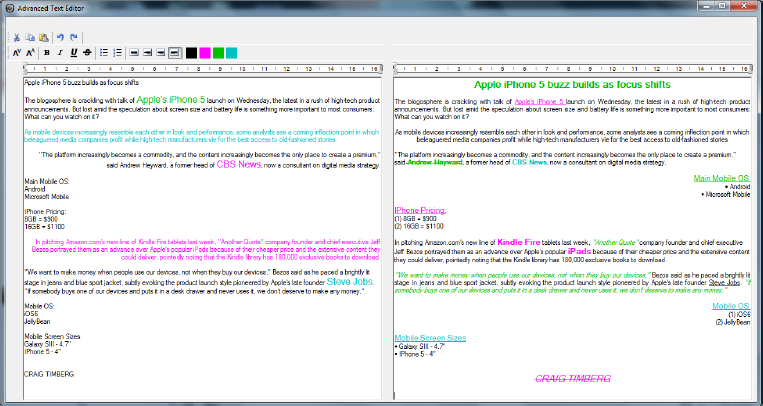
\includegraphics[width=1\linewidth]{Editor.png}
	L'interface expérimentale avec un éditeur de texte sur le côté gauche composé d'une zone de texte et d'une barre d'outils de commandes. Le format final souhaité est affiché dans la partie droite de l'éditeur de texte.
\end{center}

Les prédécesseurs ont implémenté ExposeHK. Les lettres associées aux raccourcis seront affichées lorsqu'un modificateur est appuyé (Ctrl dans ce cas).
\begin{center}
	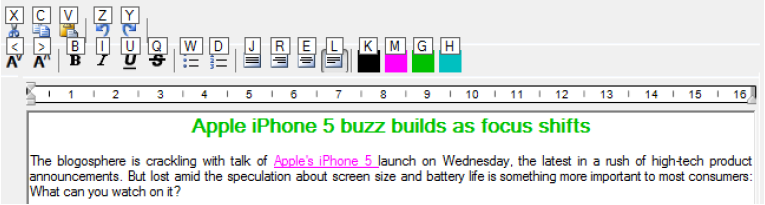
\includegraphics[width=1\linewidth]{HK.png}
	Barre d'outils avec ExposeHK activé
\end{center}
\section{Design \& Réalisation des techniques d'interaction}
Dans cette partie, la conception et la réalisation des techniques d'interaction seront introduites.
\subsection{Expose Keyboard}
Inspiré d'ExposeHK, la première technique consiste à afficher un clavier virtuel ayant tous les raccourcis de l'application lorsque l'utilisateur appuie sur le modificateur Ctrl. Dans cette technique et ExposeHK, nous fixons un délai d'affichage de 300 ms (modifiable seulement dans le code) afin de pouvoir savoir si l'utilisateur sélectionne la commande avec notre aide affichée, c'est-à-dire le clavier est affiché après 300 ms lorsque Ctrl est appuyé.
\begin{center}
	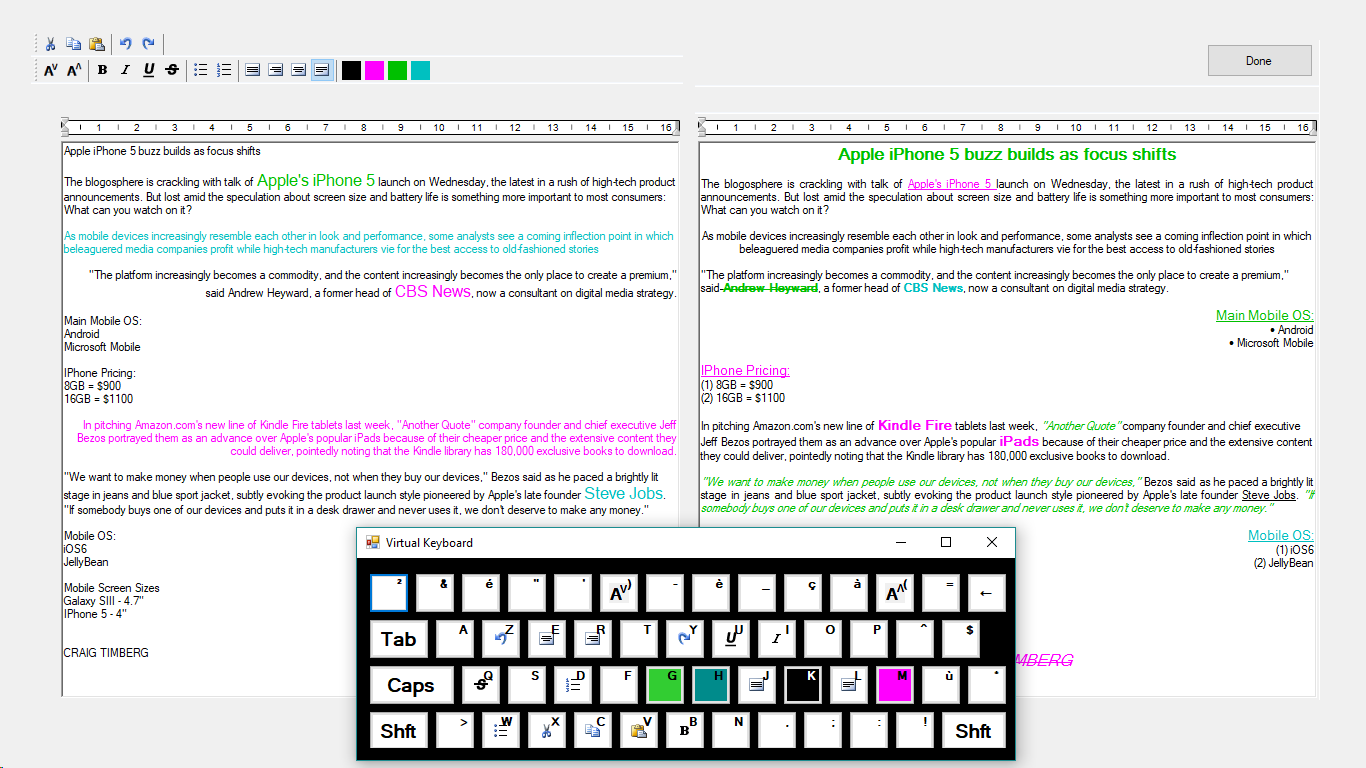
\includegraphics[width=1\linewidth]{ExposeKeyboard.png}
	Éditeur avec le clavier virtuel affiché
\end{center}
\subsection{Sticker Keyboard}
Dans un second temps, j'ai utilisé Photoshop pour redessiner et améliorer la qualité des icônes. Ensuite, elles ont été imprimées et collées sur un clavier identique à celui que je possède au laboratoire.
\begin{center}
	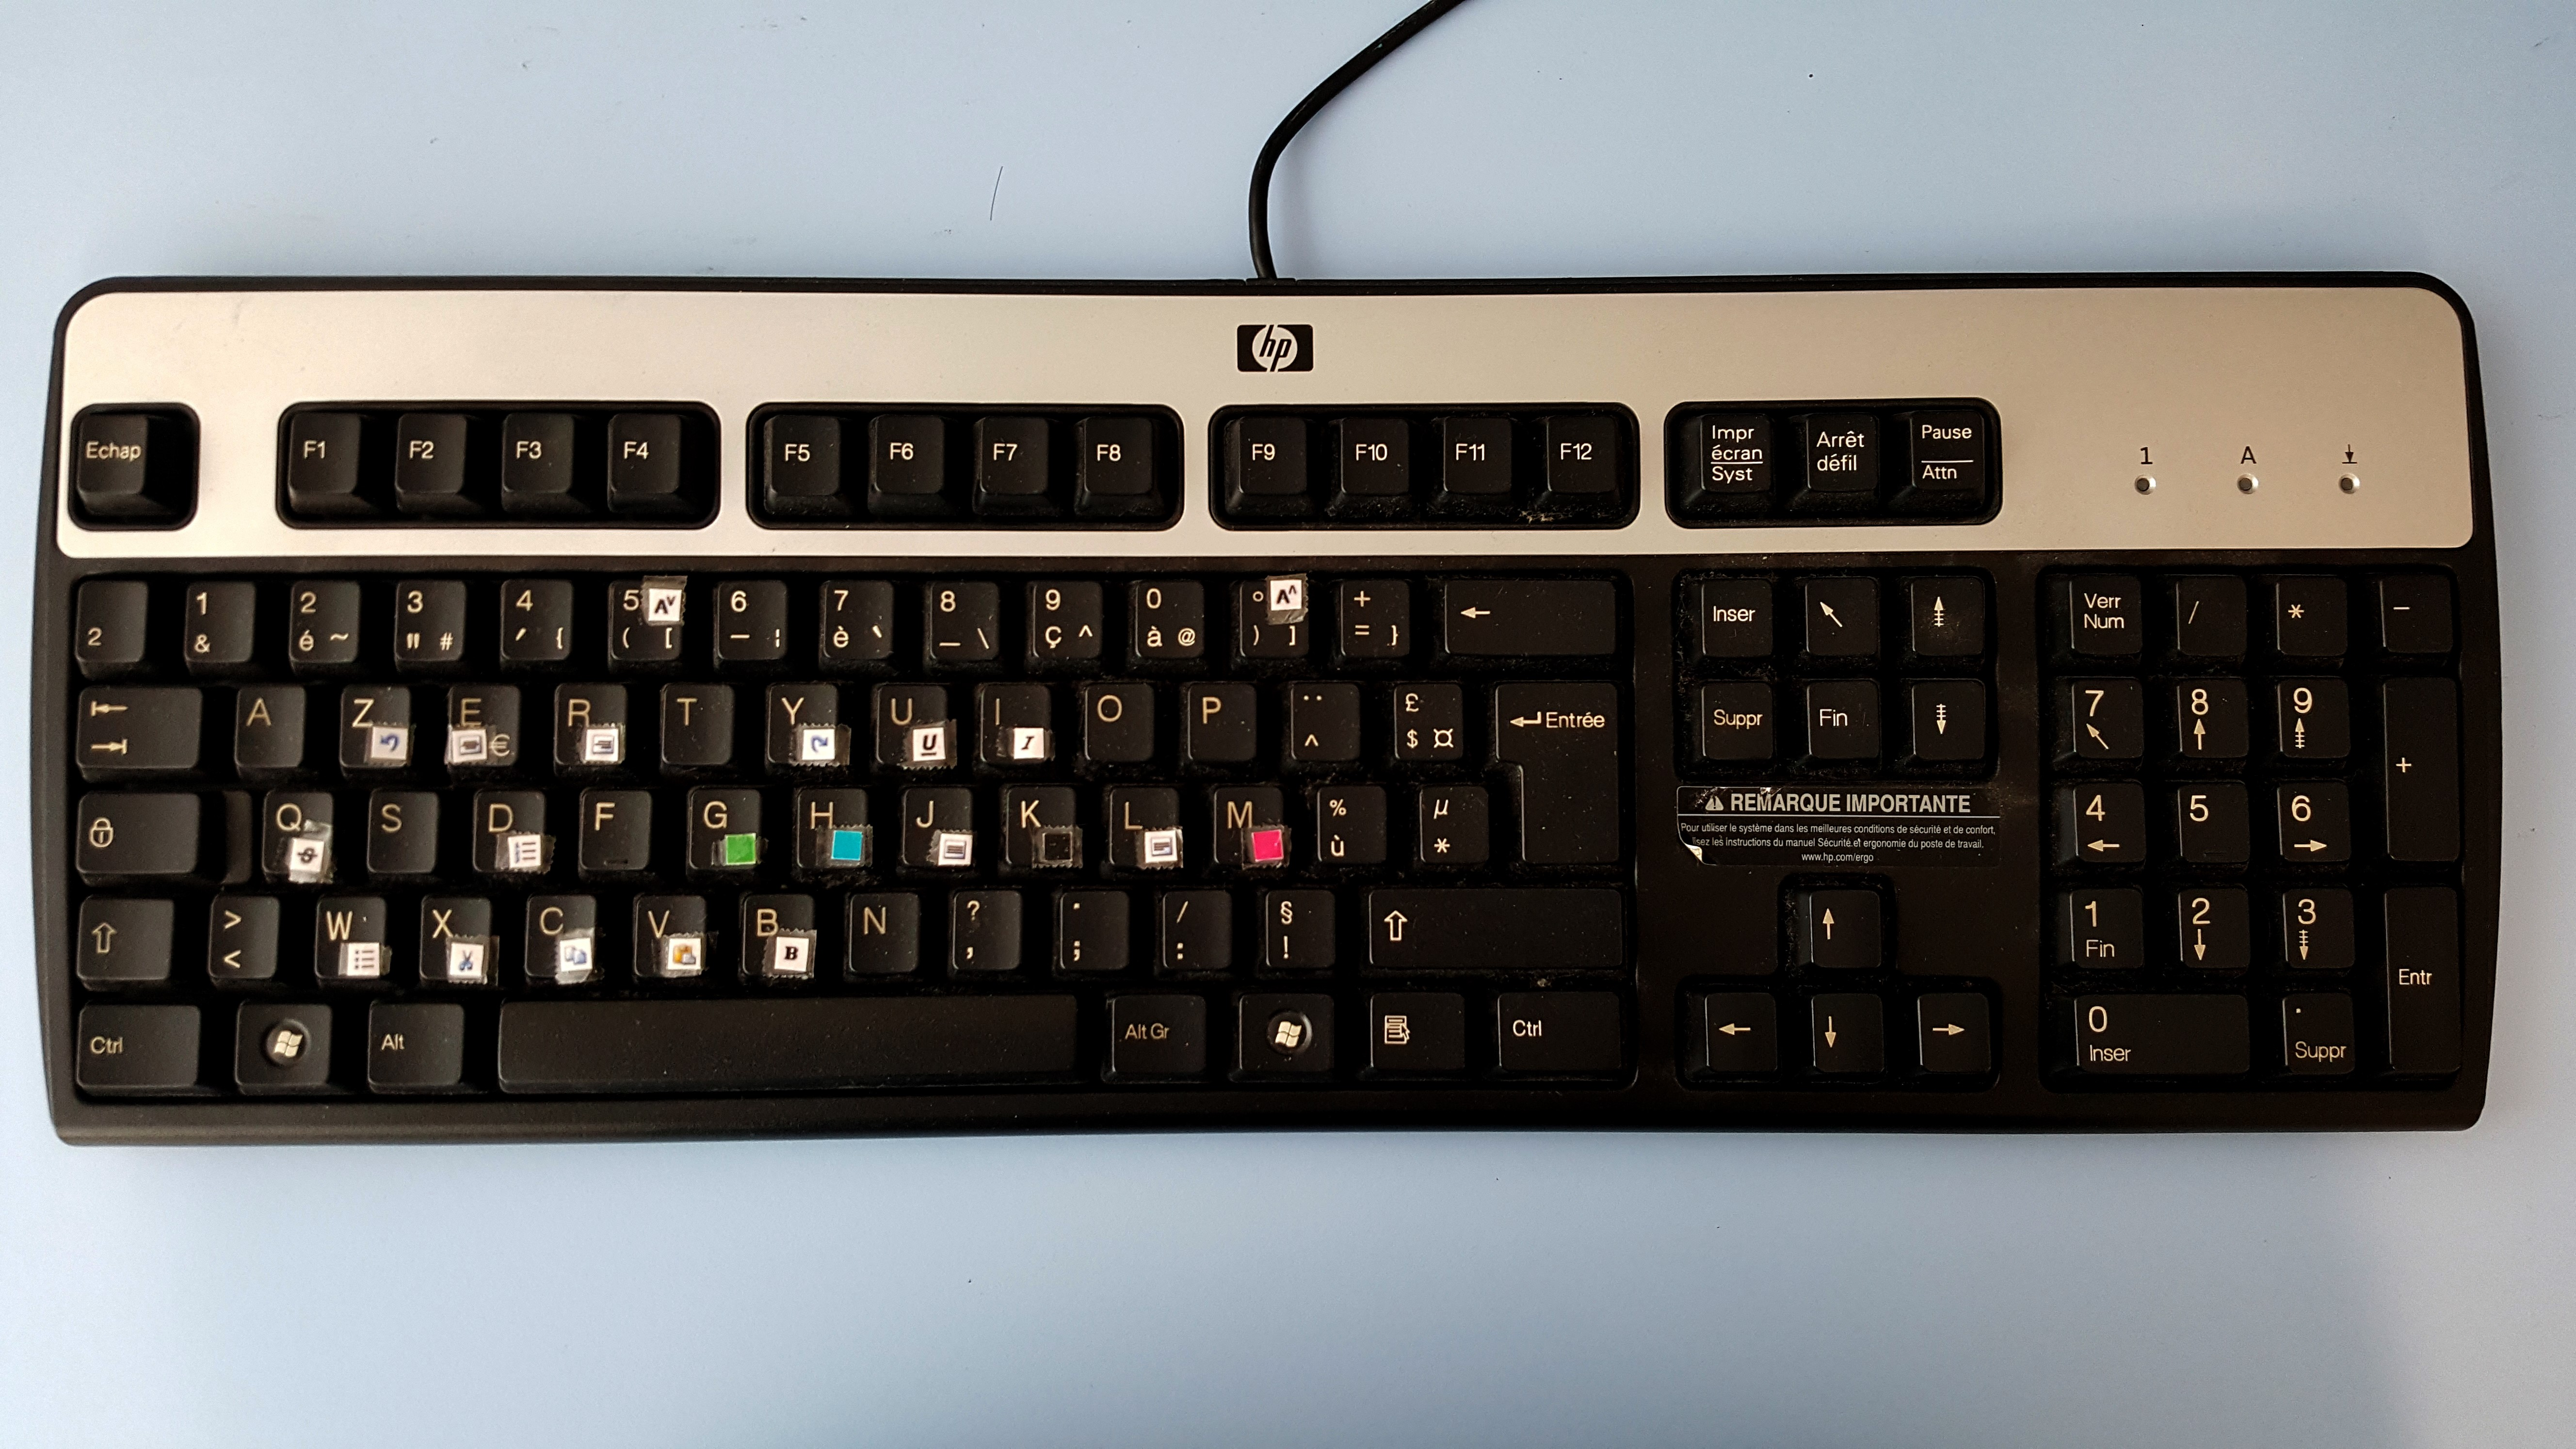
\includegraphics[width=1\linewidth]{20180723_124229.jpg}
	Clavier avec stickers
\end{center}

Cette technique se trouve pratiquement chez ceux qui doivent changer la langue mais leur clavier ne leur permet pas de visualiser les caractères, par exemple des layouts superposés pour des langues sinitiques.
\subsection{Optimus Keyboard}
La dernière technique utilise un clavier moderne avec des mini-écrans intégrés dans chaque touche qui s'appelle \href{https://www.artlebedev.com/optimus/maximus/}{Optimus Maximus} d'\href{https://www.artlebedev.com/}{Art. Lebedev Studio}. Son layout personnalisable permet une utilisation pratique de n'importe quelle langue. Il est aussi approprié pour les applications qui ont richement de raccourcis comme Photoshop ou Microsoft Word. Le fabricant dispose un forum ouvert pour des layouts personnalisés. Une application téléchargeable gratuitement est disponible sur leur site qui permet de définir de différent style pour des combinaisons des modificateurs.
\begin{center}
	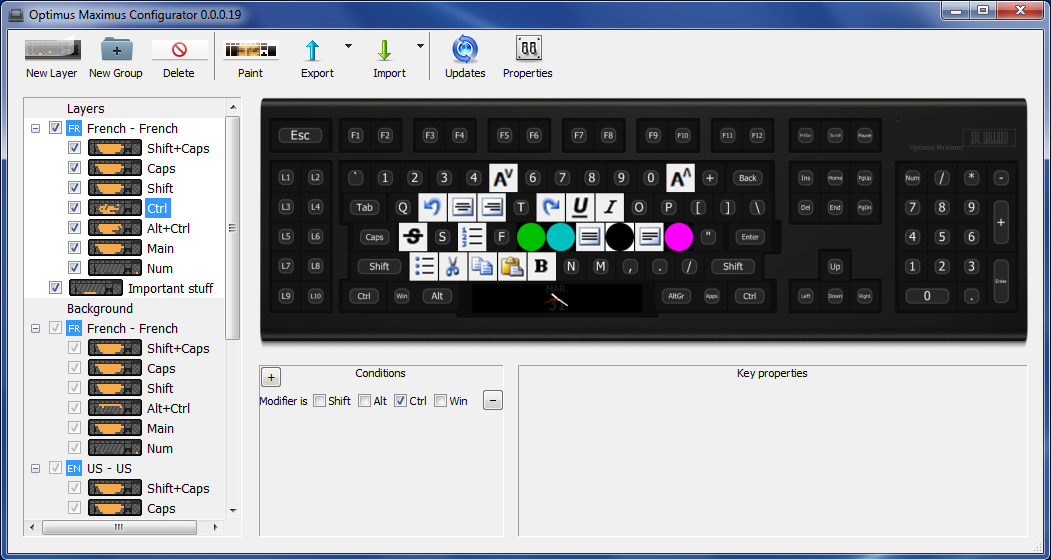
\includegraphics[width=1\linewidth]{Optimus.jpg}
	L'application fournie avec Optimus Maximus
\end{center}
\begin{center}
	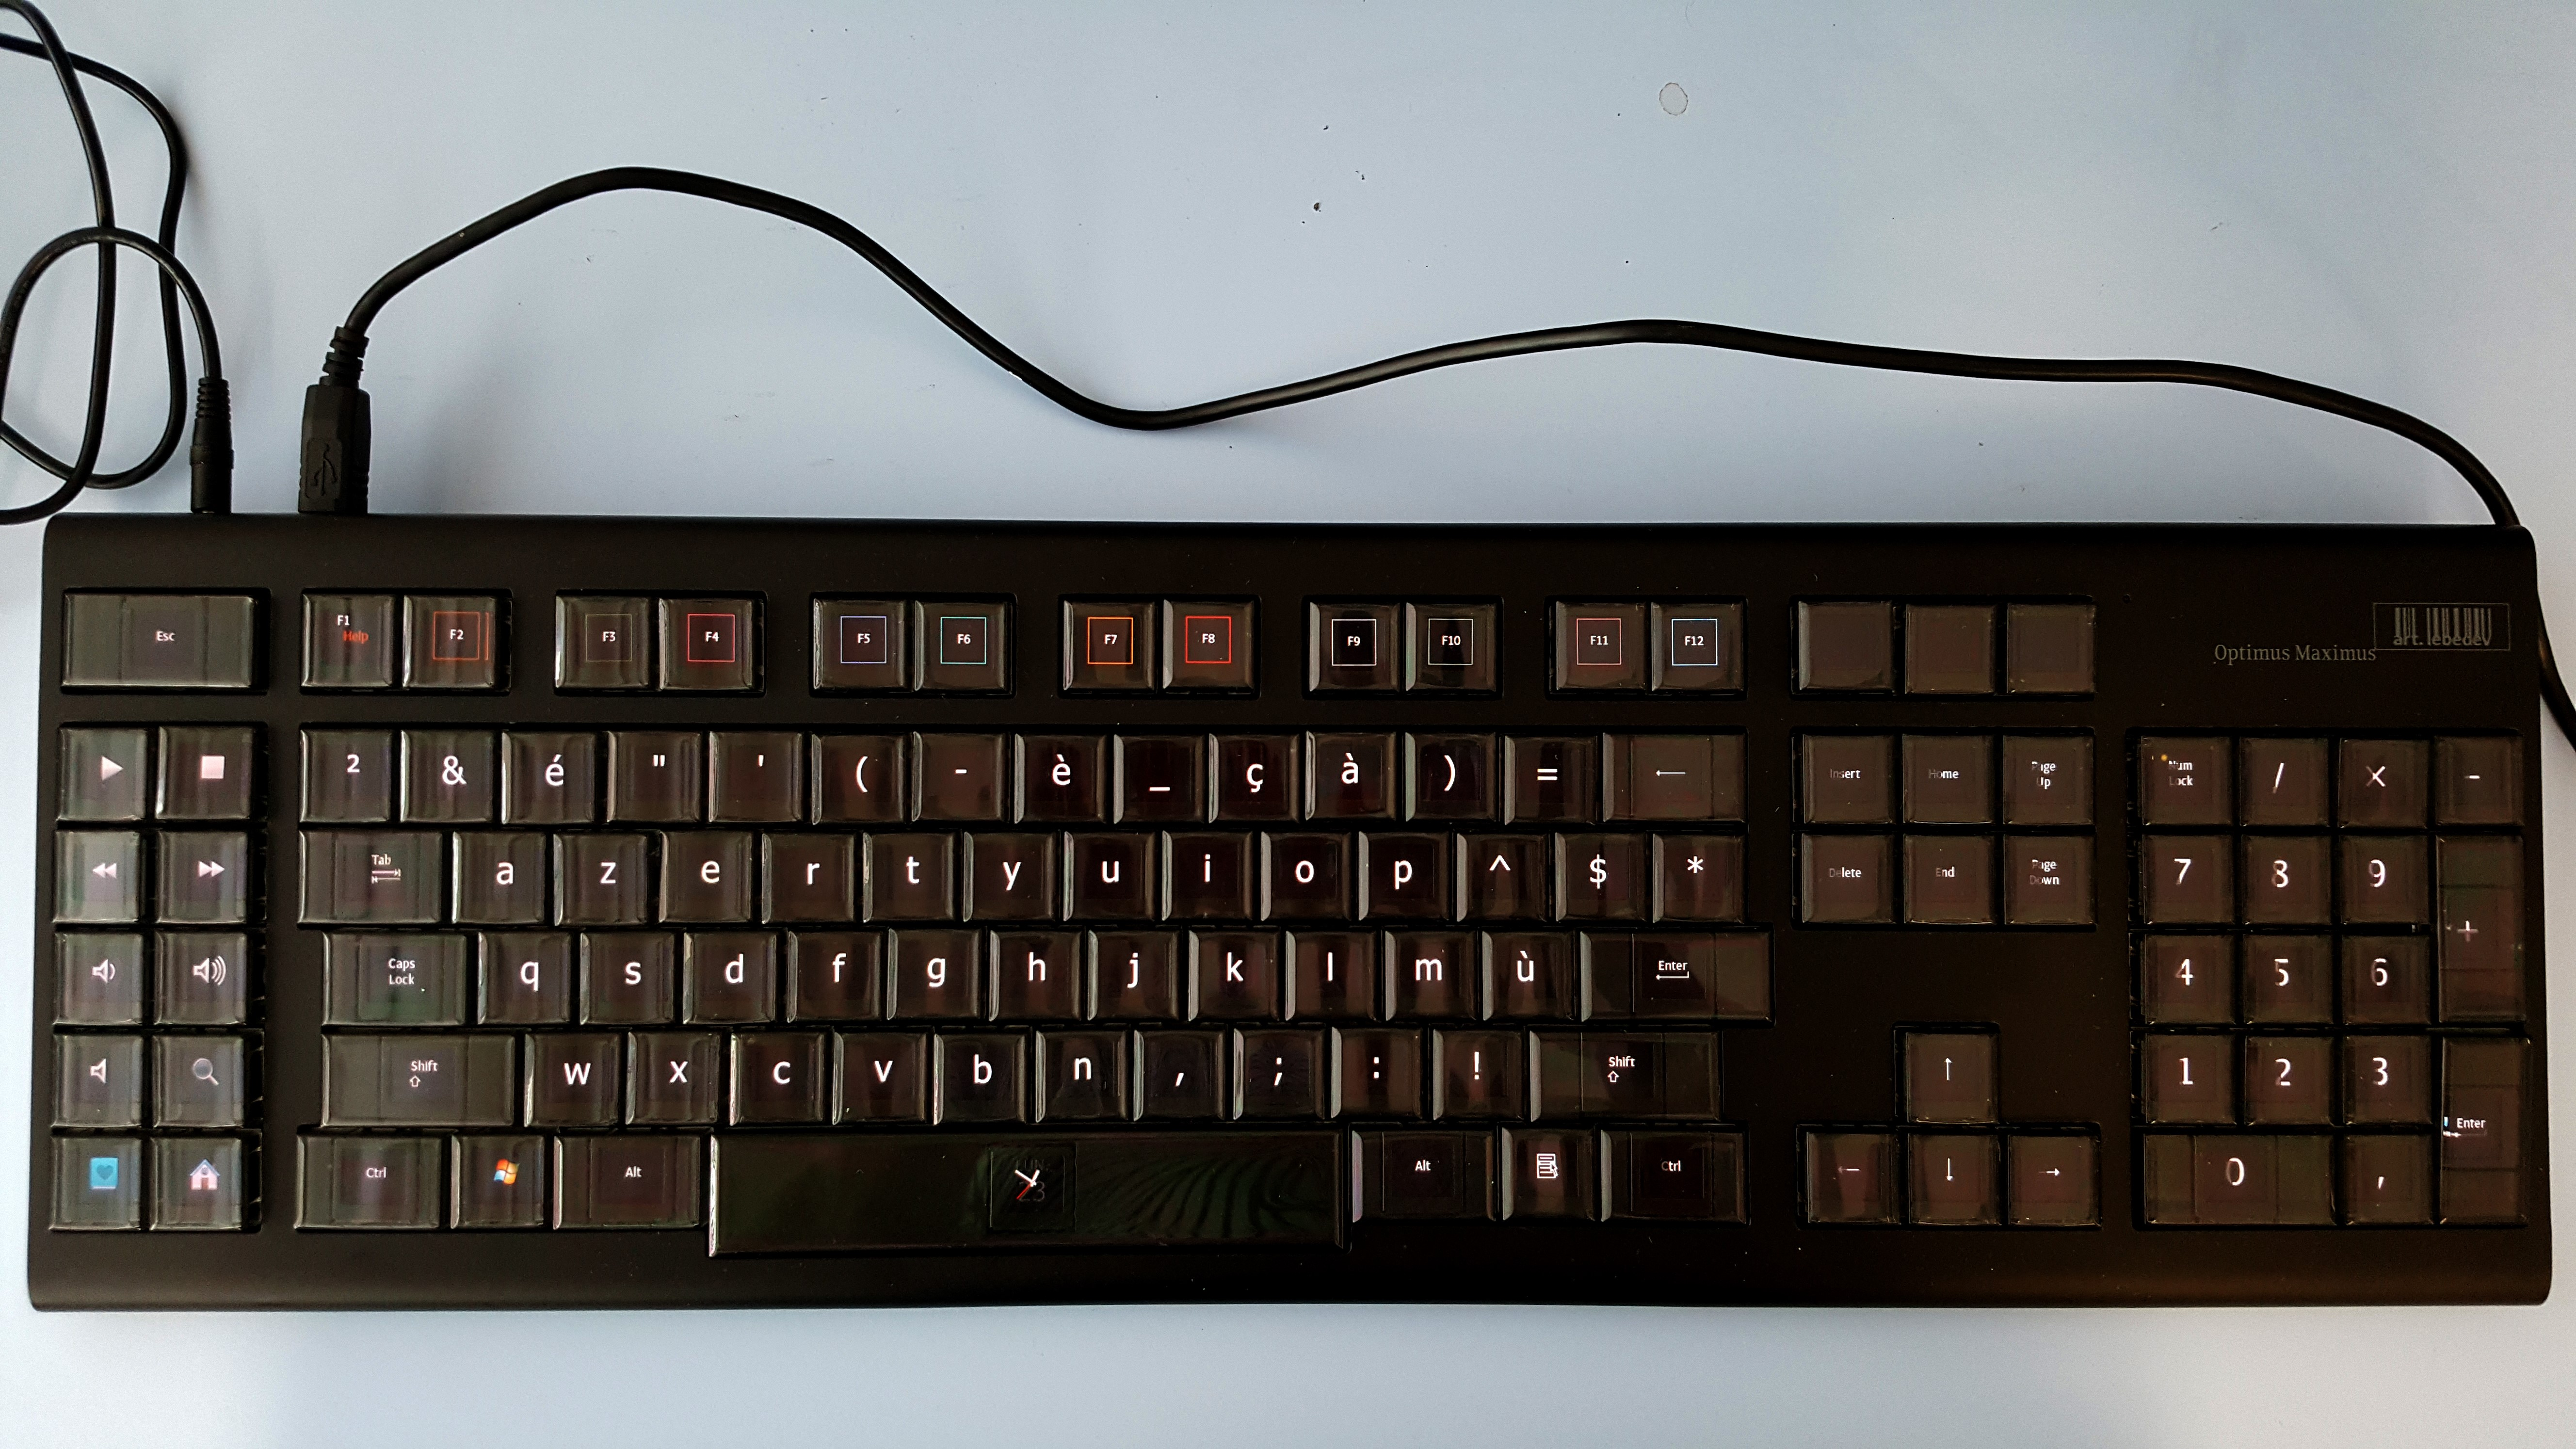
\includegraphics[width=1\linewidth]{20180723_125036.jpg}
	Optimus Maximus personnalisé en français
\end{center}
\begin{center}
	\includegraphics[width=1\linewidth]{20180723_125043.jpg}
	Optimus Maximus quand Ctrl appuyé
\end{center}
\section{Évaluation des techniques d'interaction}
\subsection{Eye Tracker}
Nous demandons aux utilisateurs leur permission d'enregistrer leurs mouvements des yeux afin de pouvoir détecter les zones d'intérêt. Nous utilisons le eye tracker de \href{https://www.tobii.com/}{Tobii} pour capturer les mouvements et logguer tous les événements de clavier et souris. 
\begin{center}
	\includegraphics[width=1\linewidth]{Tobii.jpg}
	Eye tracker utilisé dans cette expérience
\end{center}
\subsection{Étapes d'évaluation}
L'expérience se décompose en 3 phases. Dans la première phase, l'utilisateur dispose 2 blocs d'édition avec aucune aide visuelle ni physique. Il est demandé de revenir à l'ISIR au moins 48 heures après pour les phases 2 et 3. Dans la phase 2, il reformate encore 2 fois le texte qu'il avait déjà formaté lors de la première phase mais cette fois-ci avec une aide distribuée uniformément. Une fois l'édition est terminée, il est demandé de faire un test de mémorisation (phase 3). 8 personnes ont participé à cette expérience. L'application est redesignée en plein écran pour éviter les distractions.
\begin{center}
	\includegraphics[width=1\linewidth]{"Start page".png}
	L'écran d'accueil de l'application. Les phases 4 et 5 sont identiques aux phases 1 et 3 en cas de besoin de retester la mémoire ultérieurement.
\end{center}
\begin{center}
	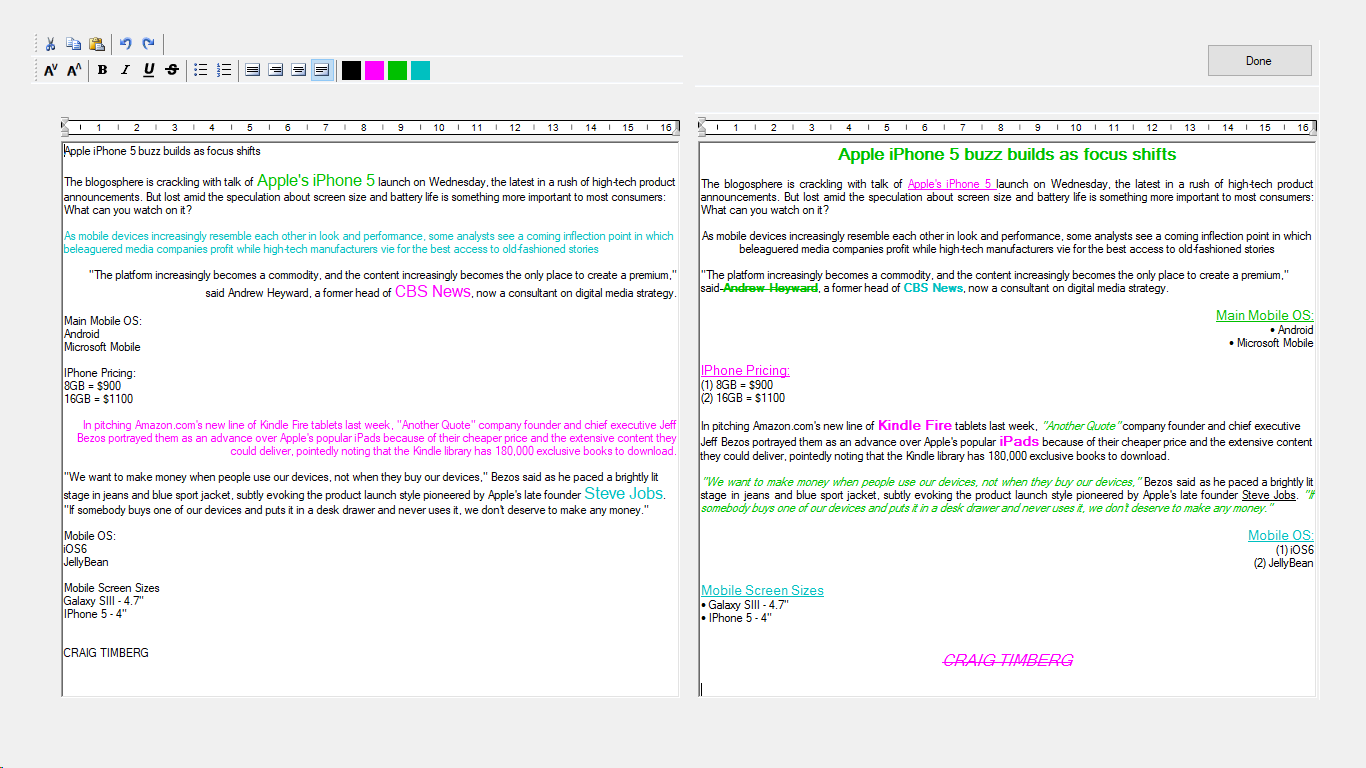
\includegraphics[width=1\linewidth]{Editor2.png}
	L'interface optimisé en séparant la bar d'outils avec l'éditeur de texte
\end{center}
\begin{center}
	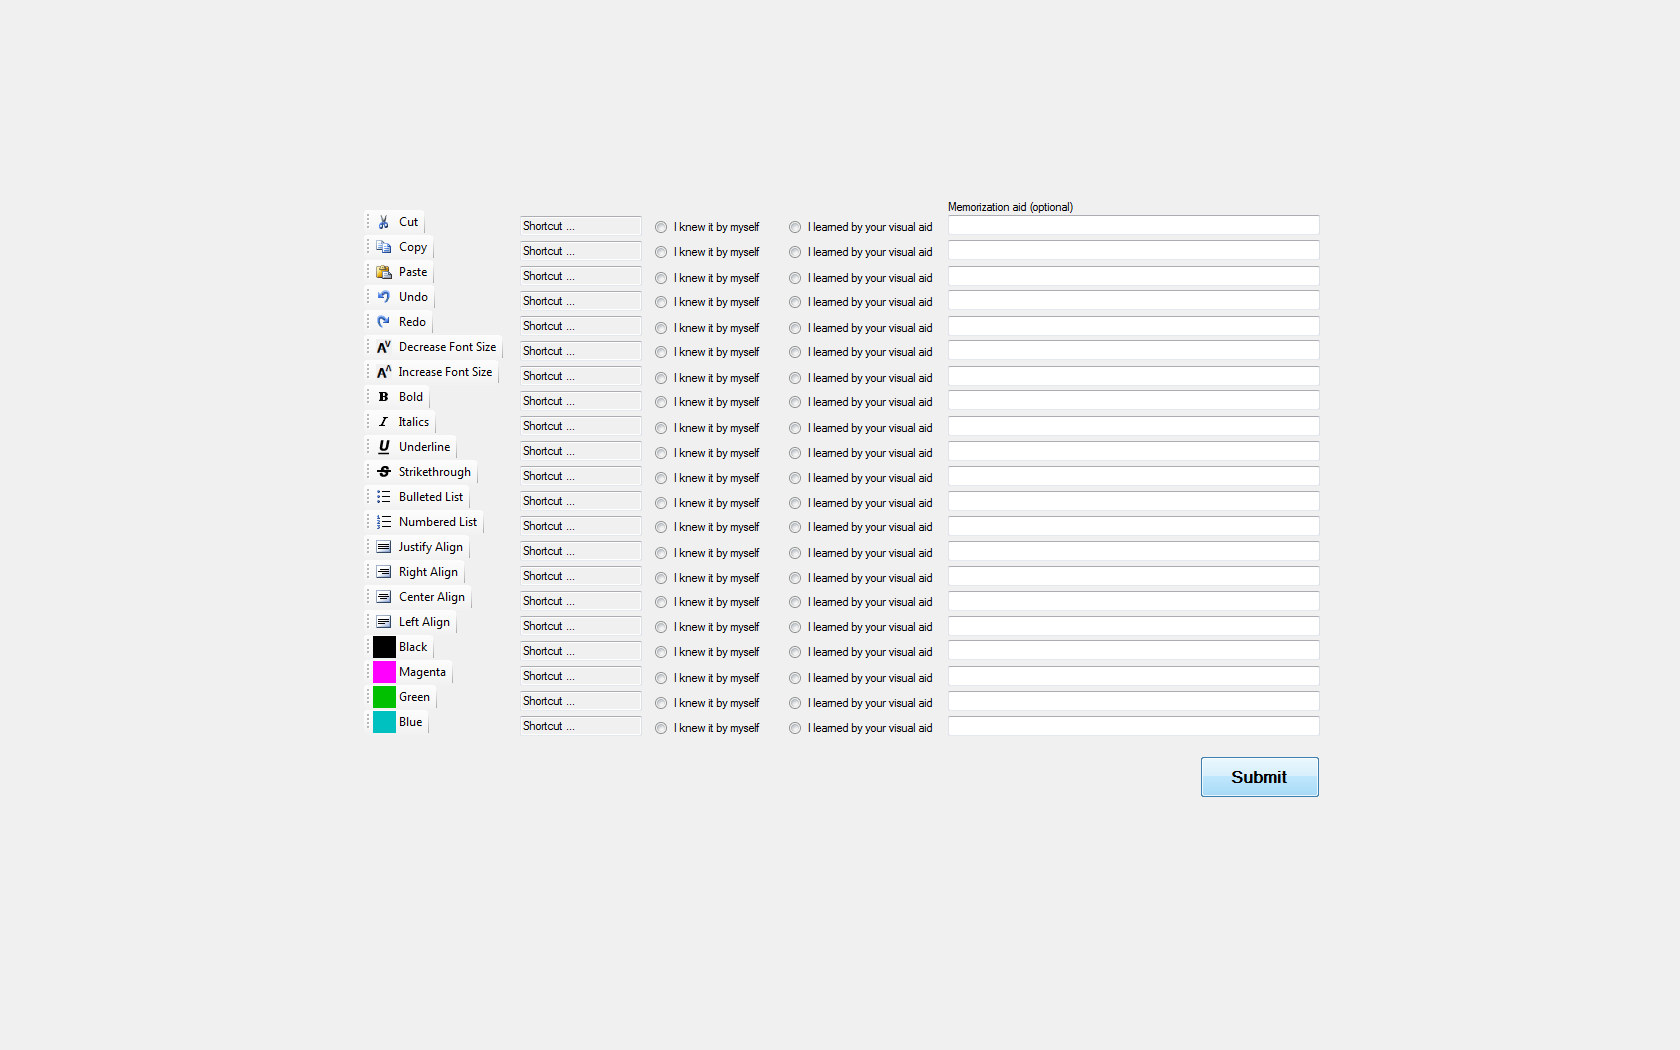
\includegraphics[width=1\linewidth]{Memo.png}
	Test de mémorisation
\end{center}
\subsection{Résultats}
Chaque technique est distribuée à une paire de participants. Nous comptons le nombre total de raccourcis retenus des participants.
\begin{center}
	\includegraphics[width=1\linewidth]{"Scores phases3 learning rate".png}
\end{center}

Nous constatons que les participants de Sticker Keyboard et ExposeHK retiennent mieux que les autres. Nous avons interrogé ceux qui ont utilisé Optimus et Expose Keyboard pour connaître la raison. Ils n'avaient pas pu se souvenir des raccourcis car les layouts sont différents. Ils ne connaissaient que la zone du lettre du raccourci. Le layout du clavier original ne correspond pas à ceux du clavier Optimus ni le clavier virtuel. En plus, les participants d'Optimus ne voient que les icônes quand ils appuient sur le modificateur, ils ne peuvent plus détecter les lettre cachées sous les icônes. Le nombre de raccourcis qu'ils ont appris au cours de l'expérience est le suivant :
\begin{center}
	\includegraphics[width=1\linewidth]{"Scores phases3 learning".png}
\end{center}

Le schéma ci-dessus montre que les participants de Sticker Keyboard ont un très bon départ avec la connaissance de plus que la moitié des commandes. Il montre également que les participants d'ExposeHK ont mieux appris les nouveaux raccourcis par rapport aux autres.

Fondamentalement, les participants de Sticker Keyboard sont avantageux dans cette expérience. C'est la raison pour laquelle ils sont très rapides bien que le temps d'édition ne soit pas le plus important critère.
\begin{center}
	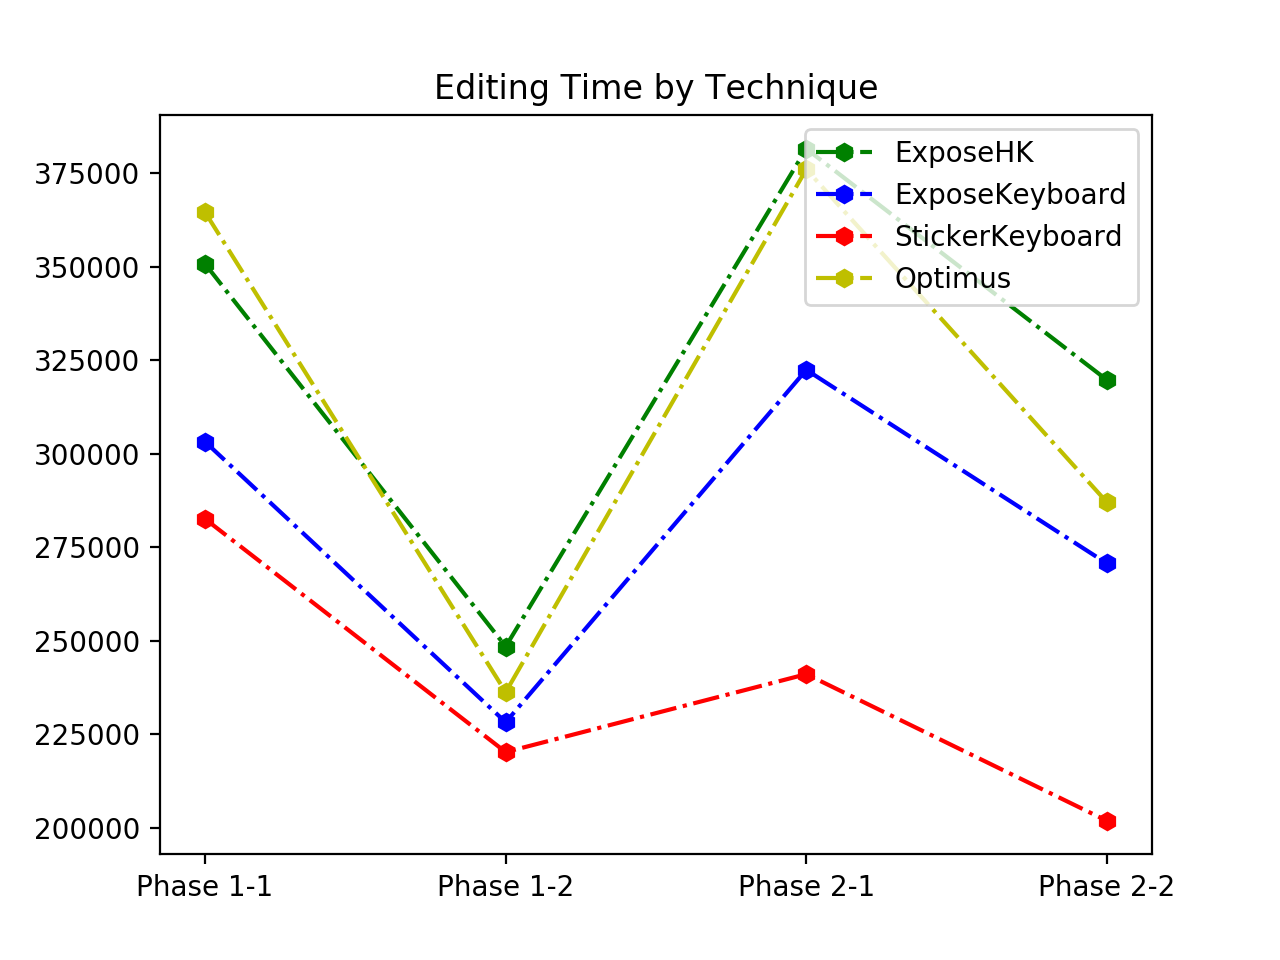
\includegraphics[width=1\linewidth]{TimeTechnique.png}
\end{center}

Un des critères importants dans cette expérience est le taux d'utilisation des raccourcis. Dans le schéma ci-dessous, nous constatons que les participants ont beaucoup utilisé des raccourcis dans la phase 2 lorsqu'ils disposaient les aides.
\begin{center}
	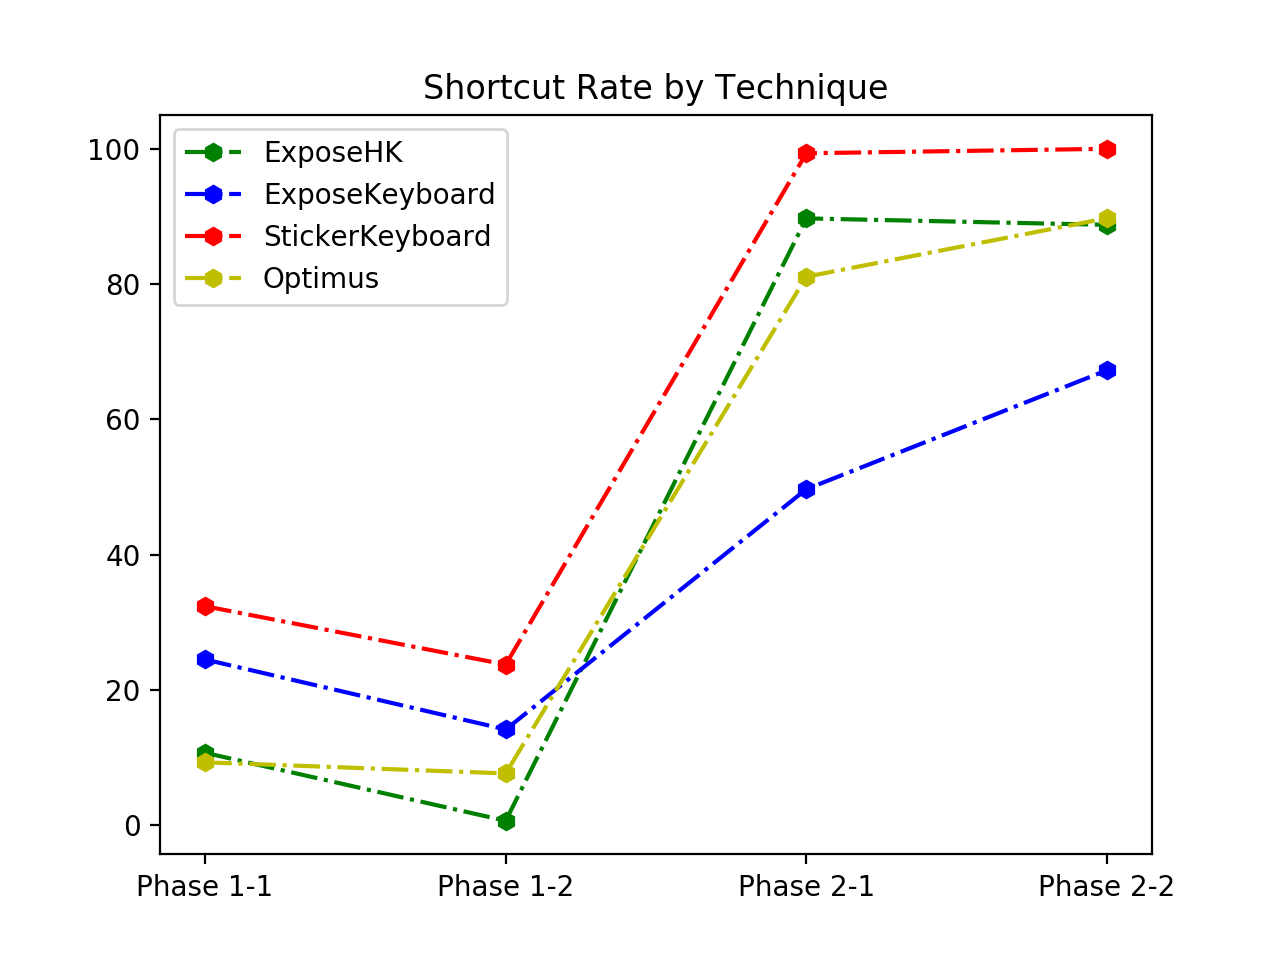
\includegraphics[width=1\linewidth]{RateTechnique.png}
	
	Le taux d'utilisation des raccourcis pour appliquer des commandes
	\includegraphics[width=0.9\linewidth]{"Rate without aid Technique".png}
	
	Le taux d'utilisation des raccourcis sans les aides visuelles pour appliquer des commandes
\end{center}

Après l'expérience, tous les participants admettent qu'ils s'intéressent plus aux commandes de base que les commandes rarement utilisées telles que la police, la numérotation et les puces, et notamment celles appliquées seulement dans notre application comme la couleur. Cela correspond strictement au résultat que nous avons obtenu.
\begin{center}
	\includegraphics[width=0.9\linewidth]{"Shortcut retrievement".png}
	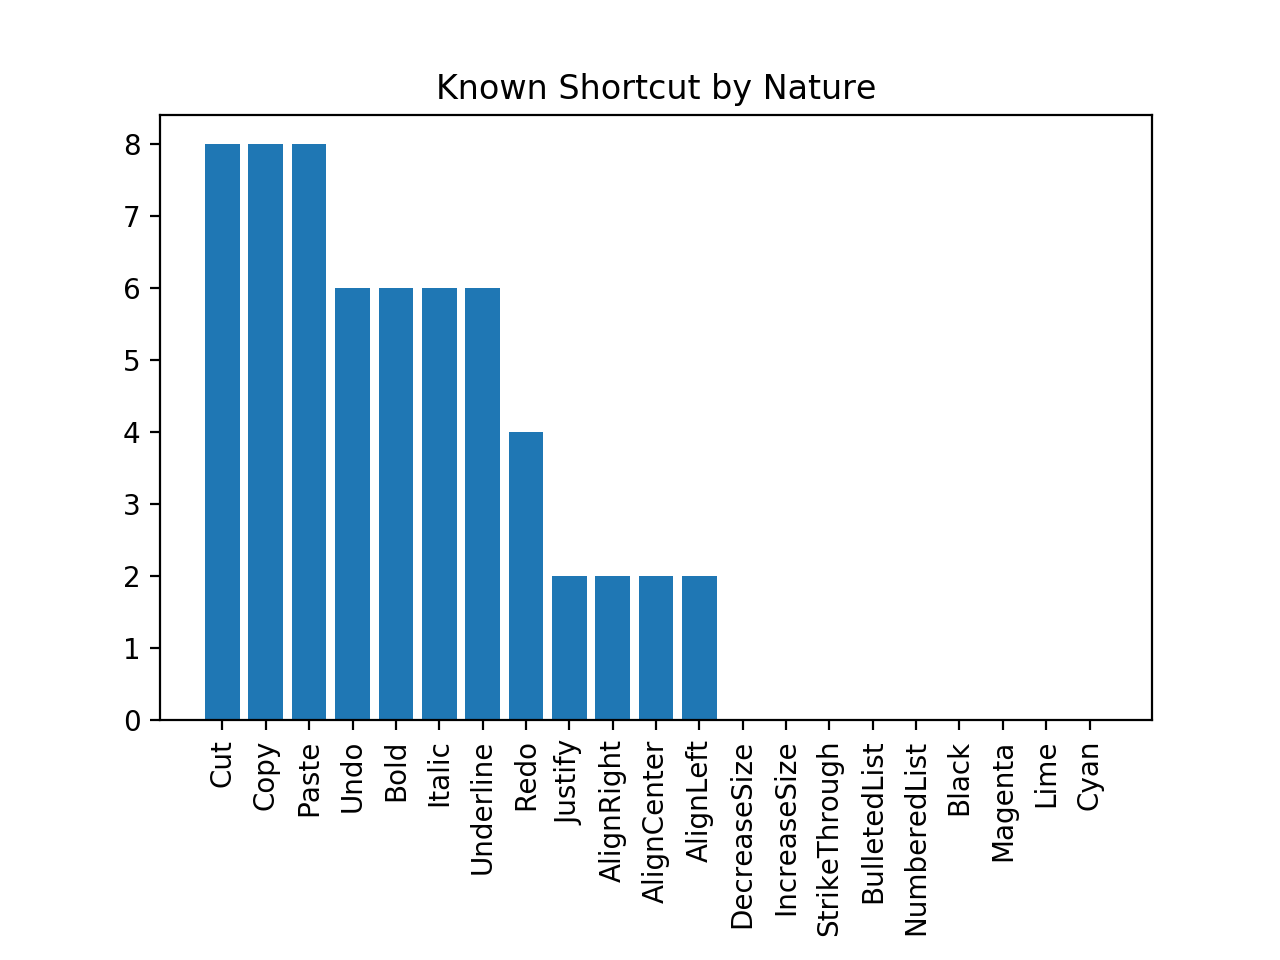
\includegraphics[width=0.9\linewidth]{Nature.png}
\end{center}
\subsection{Évaluation critique}
Bien que la différence entre les techniques soit claire, le résultat n'est pas exhaustif. Nous partons d'un déséquilibre de la qualité des participants. Le groupe de Sticker Keyboard est plus fort que celui qui utilisait le clavier Optimus. Le résultat du groupe Optimus peut s'améliorer en redesigner le layout en mettant les lettres avec les icônes. La taille de l'échantillon est aussi petite suite au temps restreint. Il faudra donc continuer ce projet en augmentant le nombre de participants. Plus grande la taille de l'échantillon, plus précis sera le résultat. Les données du tracker devraient être explorées pour pouvoir être capable de analyser plus profondément.
\section{Conclusion}
Ce stage est une expérience enrichissante pour moi. J'apprécie d'avoir fait partie d'une équipe dynamique et accueillante et d'avoir connu l'environnement de travail international dans un laboratoire de recherche. Grâce à ce stage, j'ai pu améliorer mes compétences sociales et élargir mes connaissances.

Le projet est une bonne expérience pour moi. En effet, je ne connaissais le langage C\# avant le stage qui est omniprésent dans les entreprises. Malgré que le résultat n'est pas exhaustif, il m'a donné une méthode d'analyse structurelle et une nouvelle perspective dans le domaine interaction
\newpage
\begin{thebibliography}{10}
	\bibitem{1} A. Cockburn, C. Gutwin, J. Scarr, et S. Malacria, «Supporting Novice to Expert
	Transitions in User Interfaces», \textit{ACM Comput. Surv.}, vol. 47, n\textdegree\ 2, p. 31:1–31:36, nov. 2014.
	\bibitem{2} J. Harrison, «Improving Users' Command Selection Performance», p.30-35, nov. 2012.
	\bibitem{3} S. Malacria, G. Bailly, J. Harrison, A. Cockburn, et C. Gutwin, «Promoting Hotkey Use
	Through Rehearsal with ExposeHK», in \textit{Proceedings of the SIGCHI Conference on Human Factors in Computing Systems}, New York, NY, USA, 2013, p. 573–582.
\end{thebibliography}
\end{document}